\label{chapter:evaluation:tests}

We have designed several test scenes to test various aspects of the final API. The tests scenarios are used for obtaining source code metrics, as well as for performance comparison between the implementations with and without the PURGE layer.

All source code measurements exclude statements in reference engines that have no equivalence in the simplified PURGE API. Furthermore, many test scenarios include source code from previous tests. To keep the focus on the current test, all statements that were covered in a prior case are ignored.

The measured values are:

\begin{smalllist}
	\item Lines of code: Number of lines in the source code of the application. Each line contains a single statement, empty lines and lines consisting of a single brace are ignored. Some tests further do not include the placement of a camera, which is required to test the number of rendered frames per second (below), thus the statements required for this positioning are ignored, too.
	\item Function calls: Number of API functions that were used for the implementation.
	\item Distinct function calls: This value represents the number of different functions that were needed to implement the scenario. It is assumed that a lower value reduces the complexity of the API.
	\item Average frames per second: Number of frames that were drawn until the end of the test application. The value is the average of 100 runs of the test scenario, rendering for five seconds in each iteration. It is important to note that this value is highly dependent on the bridge implementation in the case of PURGE.
	\item Peak memory usage: This value is obtained through the \inlinecode{getrusage()} system call on Linux.
\end{smalllist}

\section{Creating a scene}

The first 5 test cases will gradually create an application that will render a space ship at the center of the render window. The finished scene is depicted in figure \ref{fig:TestScene5}

\begin{figure}[htbp]
	\centering
	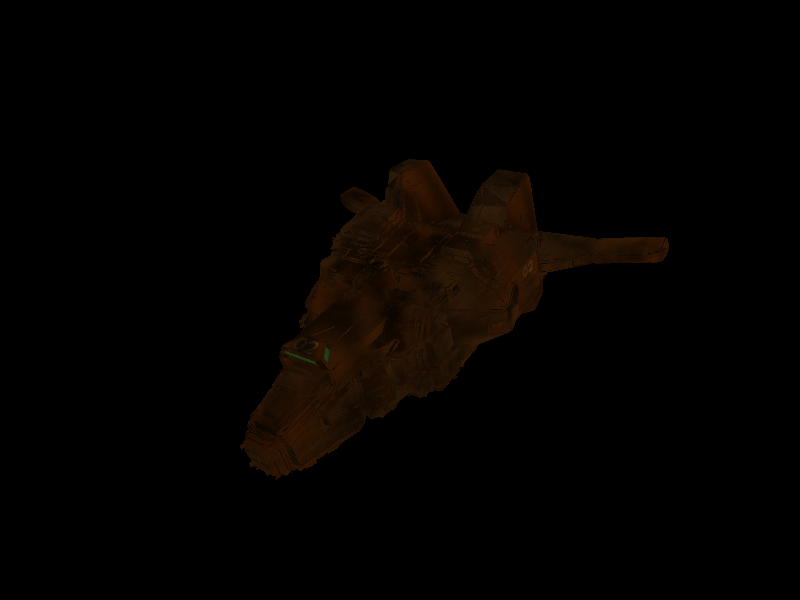
\includegraphics[width=10cm]{images/TestScene5.png}
	\caption{Output of TestScene5}
	\label{fig:TestScene5}
\end{figure}

\subsection{TestScene1: Creating an empty render window}

	The minimal code required to create a window and enter a render loop that will exit whenever the window is closed. This is the most basic scenario for every graphics engine. This test measures the load of the boilerplate code of each graphics library. A performance comparison is not sensible in this case, as PURGE chooses to create a differently sized default render window than Ogre3d.
	
	\begin{table}[htpb]
		\center
		\caption{Code metrics for TestScene1}
		\begin{tabular}{l | l | l | l | l}
			& PURGE & Ogre3d & OpenSceneGraph & Panda3d \\ \hline
			Lines of Code & 2 & 8 & 1 & 4\\
			Function calls & 3 & 9 & 2 & 4\\
			Distinct Function calls & 3 & 9 & 2 & 4\\
		\end{tabular}
		\label{tbl:Code1}
	\end{table}

	Table \ref{tbl:Code1} shows that OpenSceneGraph needs the fewest lines of code for this task. PURGE has two semantically equivalent statements but requires an additional call for the instantiation of the \classname{Renderer}. Additionally this test provides the first assertion of the initial statement that Ogre3d is quite verbose.

\subsection{TestScene2: Controlling the render window}

	In order to create a test scene that allows direct comparison of the frame rates of the same application with and without the PURGE layer, the render window will be adjusted in this test: The render window is centered on the display and created with a predefined size of 800x600 pixels. Panda3d is the only library that did not need the render window object in the initial test case. The results can be seen in Table \ref{tbl:Code2}.

	\begin{table}[htpb]
		\center
		\caption{Code metrics for TestScene2}
		\begin{tabular}{l | l | l | l | l}
			& PURGE & Ogre3d & OpenSceneGraph & Panda3d\\ \hline
			Lines of Code & 1 & 1 & 1 & 3\\
			Function calls & 1 & 1 & 1 & 3\\
			Distinct Function calls & 1 & 1 & 1 & 3\\
		\end{tabular}
		\label{tbl:Code2}
	\end{table}

	This test is the first to additionally measure impact of the added layer to the rendering performance (Table \ref{tbl:Performance2}). As the scene is completely empty (no visible objects have been created), this value shows the resource usage for the idle render loop. This already-low value will further decrease as the impact of the render loop itself is negligible in a graphics application.
	
	\begin{table}[htpb]
		\center
		\caption{Performance metrics for TestScene2}
		\begin{tabular}{l | l | l | l}
			& without PURGE & with PURGE & relative value\\ \hline
			Frames per second & 8726.45 & 8713.35 & 99.85\%\\
			Peak memory usage & 76709 & 77170 & 100.60\%\\
		\end{tabular}
		\label{tbl:Performance2}
	\end{table}

\subsection{TestScene3: Positioning the camera}

	The camera is positioned at \vect{X}{X}{X} and rotated to look at the origin. Panda3d performs all required steps in one statement each:

	\begin{numlist}
		\item retrieving the camera object from the window,
		\item repositioning the camera and
		\item setting the new orientation to look at the global origin.
	\end{numlist}
	
	As OpenSceneGraph provides a method similar to GLU's \inlinecode{gluLookAt()}, the re-alignment can be performed in a single step. PURGE instead makes use of its fluent interfaces to reduce the lines of required code and Ogre3d needs to create a dedicated scene node that performs the transformation for the camera.

	\begin{table}[htpb]
		\center
		\caption{Code metrics for TestScene3}
		\begin{tabular}{l | l | l | l | l}
			& PURGE & Ogre3d & OpenSceneGraph & Panda3d\\ \hline
			Lines of Code & 1 & 3 & 2 & 3\\
			Function calls & 3 & 4 & 5 & 3\\
			Distinct Function calls & 3 & 4 & 5 & 3\\
		\end{tabular}
		\label{tbl:Code3}
	\end{table}

	The repositioning of the camera did not have any impact on the rendering performance, but the tiny gap between the measured memory consumptions closes a bit further as Ogre3d needs to make use of an additional object.

	\begin{table}[htpb]
		\center
		\caption{Performance metrics for TestScene3}
		\begin{tabular}{l | l | l | l}
			& without PURGE & with PURGE & relative value\\ \hline
			Frames per second & 8727.26 & 8712.92 & 99.84\%\\
			Peak memory usage & 76709 & 76934 & 100.29\%\\
		\end{tabular}
		\label{tbl:Performance3}
	\end{table}

\subsection{TestScene4: Loading an object}

	The next step involves loading an object into the scene without modifying its position: the object is attached to the root scene node. As attaching the object to the scene graph is implicit in PURGE, the whole task can be performed in a single step. Ogre3d needs to implement the remaining boilerplate code for registering the location of the resource.

	\begin{table}[htpb]
		\center
		\caption{Code metrics for TestScene4}
		\begin{tabular}{l | l | l | l | l}
			& PURGE & Ogre3d & OpenSceneGraph & Panda3d\\ \hline
			Lines of Code & 1 & 4 & 1 & 2\\
			Function calls & 1 & 6 & 2 & 4\\
			Distinct Function calls & 1 & 6 & 2 & 4\\
		\end{tabular}
		\label{tbl:Code4}
	\end{table}

	The object used for this test consists of approximately 123.000 triangles. We had assumed that the performance difference would decrease in previous tests and this assumption is backed by the performance difference presented in Table \ref{tbl:Performance4}. The memory footprint of the loaded object further reduces the difference in memory consumption.

	\begin{table}[htpb]
		\center
		\caption{Performance metrics for TestScene4}
		\begin{tabular}{l | l | l | l}
			& without PURGE & with PURGE & relative value\\ \hline
			Frames per second & 661.75 & 660.92 & 99.87\%\\
			Peak memory usage & 145362 & 145446 & 100.06\%\\
		\end{tabular}
		\label{tbl:Performance4}
	\end{table}

\subsection{TestScene5: Positioning after loading}

	The previously loaded object is now positioned at the coordinates \vect{-X}{-X}{-X}. Ogre3d and OpenSceneGraph need to create a new scene node that accepts this transformation. A model in Panda3d is itself a scene node that can be manipulated directly. The implementation using PURGE makes use of the fluent interface to append a single function call to an existing line.

	\begin{table}[htpb]
		\center
		\caption{Code metrics for TestScene5}
		\begin{tabular}{l | l | l | l | l}
			& PURGE & Ogre3d & OpenSceneGraph & Panda3d\\ \hline
			Lines of Code & 0 & 2 & 4 & 1\\
			Function calls & 1 & 3 & 4 & 1\\
			Distinct Function calls & 1 & 3 & 4 & 1\\
		\end{tabular}
		\label{tbl:Code5}
	\end{table}

	The additional scene node required by Ogre3d further closes the performance gap between the two implementations, whereas the difference in memory consumption does not change at all.

	\begin{table}[htpb]
		\center
		\caption{Performance metrics for TestScene5}
		\begin{tabular}{l | l | l | l}
			& without PURGE & with PURGE & relative value\\ \hline
			Frames per second & 670.15 & 669.96 & 99.97\%\\
			Peak memory usage & 145361 & 145446 & 100.06\%\\
		\end{tabular}
		\label{tbl:Performance5}
	\end{table}

\section{Completed Scene}

	So far we have looked at the complexity of very specific, incremental tasks. To get a better overview on the amount of code required for the whole scene, we will additionally consider the code metrics of the complete application we have created step by step during the previous five test cases. Table \ref{tbl:Complete5} shows the difference between all APIs.

	\begin{table}[htpb]
		\center
		\caption{Code metrics for the whole TestScene5 implementation}
		\begin{tabular}{l | l | l | l | l}
			& PURGE & Ogre3d & OpenSceneGraph & Panda3d\\ \hline
			Lines of Code & 5 & 19 & 10 & 12\\
			Function calls & 8 & 23 & 14 & 16\\
			Distinct Function calls & 7 & 21 & 14 & 14\\
		\end{tabular}
		\label{tbl:Complete5}
	\end{table}

\section{Modification over time}

	As the previous tests were testing the creation of a single, static scene, we will be looking at some dynamically updated scene graphs in this section.

	\subsection{TestScene6: Movement}

		This scene implements a straight movement of a previously loaded object from one point to another. The presence of the automatic scene node manipulator simplifies this task tremendously in the application using PURGE. The Panda3d API is satisfied with a single function, the other implementations need a separate class for an ongoing modification of the scene. In either case the implementation drives the developer through a lot more knowledge than necessary for such a simple task.

		The metrics just count the amount of effort required to implement this feature into an existing scene. We will only be measuring the statements we needed to write to make the object in TestScene5 move.

		\begin{table}[htpb]
			\center
			\begin{tabular}{l | l | l | l | l}
				& PURGE & Ogre3d & OpenSceneGraph & Panda3d\\ \hline
				Lines of Code & 1 & 8 & 8 & 5\\
				Function calls & 4 & 11 & 12 & 8\\
				Distinct Function calls & 4 & 11 & 12 & 8\\
			\end{tabular}
			\caption{Code metrics for TestScene6}
		\end{table}

		The performance difference between the two implementations was rather small again.

		\begin{table}[htpb]
			\center
			\caption{Performance metrics for TestScene6}
			\begin{tabular}{l | l | l | l}
				& without PURGE & with PURGE & relative value\\ \hline
				Frames per second & 668.50 & 668.22 & 99.96\%\\
				Peak memory usage & 145361 & 145454 & 100.06\%\\
			\end{tabular}
			\label{tbl:Performance6}
		\end{table}

	\subsection{TestScene7: Rotation}

		This test scene implements a 360\degree rotation of an existing object. As with the previous test we will only measure the additional statements required for the rotation. Not surprisingly, the results are very similar to that of the previous test.

		\begin{table}[htpb]
			\center
			\begin{tabular}{l | l | l | l | l}
				& PURGE & Ogre3d & OpenSceneGraph & Panda3d\\ \hline
				Lines of Code & 1 & 10 & 8 & 7\\
				Function calls & 4 & 14 & 11 & 11\\
				Distinct Function calls & 4 & 14 & 11 & 11\\
			\end{tabular}
			\caption{Code metrics for TestScene7}
		\end{table}

		\begin{table}[htpb]
			\center
			\caption{Performance metrics for TestScene7}
			\begin{tabular}{l | l | l | l}
				& without PURGE & with PURGE & relative value\\ \hline
				Frames per second & 670.38 & 670.27 & 99.98\%\\
				Peak memory usage & 145365 & 145458 & 100.06\%\\
			\end{tabular}
			\label{tbl:Performance7}
		\end{table}

\section{Scalability tests}

	The next few tests will probe how the library behaves when the amount of objects increases. As the tests merely add some loops into the previously analyzed code, we will omit the code metrics for the next tests and just look at the performance. To keep the focus further on the CPU-operations, we have performed all tests in this chapter with cubes of size \vect{1}{1}{1}. More complex objects would shift the majority of the execution onto the GPU, which does the exact same operations in both implementations.

	\subsection{TestScene8: Many objects at origin}

		We have created one thousand cubes at the origin of a scene for this test. The Ogre3d implementation attaches all objects directly to the root scene node, whereas the \classname{Renderer} of PURGE creates a dedicated scene node for each object. The results clearly show that these additional scene nodes have a huge impact on the performance in the Ogre3d rendering process. The additional nodes further result in increased memory consumption.

		\begin{table}[htpb]
			\center
			\caption{Performance metrics for TestScene8}
			\begin{tabular}{l | l | l | l}
				& without PURGE & with PURGE & relative value\\ \hline
				Frames per second & 872.94 & 32.84 & 3.76\%\\
				Peak memory usage & 64806 & 68778 & 106.13\%\\
			\end{tabular}
			\label{tbl:Performance8}
		\end{table}

		This is an uncommon use case scene in graphics development, as there are usually very few objects attached to the root scene node. These are the objects that form the immobile environment of the scene -- like the plants and rocks provided by Panda3d's official tutorial application, depicted in Figure \ref{fig:TiltedCamera}. On the other hand, these models can be extremely complex, straining the GPU in another way. To assess these thoughts, we have created the same test scene with a single, complex object, Ogre3d's official ogre head model consisting of 2242 vertices.
		
		\begin{table}[htpb]
			\center
			\caption{Performance metrics for TestScene8.2}
			\begin{tabular}{l | l | l | l}
				& without PURGE & with PURGE & relative value\\ \hline
				Frames per second & 625.87 & 630.57 & 100.75\%\\
				Frames per second (no far-clipping) & 632.73 & 629.06 & 99.42\%\\
				Peak memory usage & 68229 & 68356 & 100.19\%\\
			\end{tabular}
			\label{tbl:Performance8.2}
		\end{table}

		Interestingly, PURGE achieved a higher frame rate in this test. This unexpected difference was caused by the default values of the camera frustum in PURGE: we have disabled the far end of the frustum, always drawing everything in sight. This will generate much worse results with a more populated scene, but we will keep the implication that such a scene will require manual tweaking of the camera parameters, optimizing the API for the simplest scenes. Re-running the application after adjusting the Ogre3d implementation provided the results in Table \ref{tbl:Performance8.2}. We have added this newly found optimization to all following tests.

		The elaboration on the initial test showed that the PURGE software layer has trouble with multitudes of objects positioned at the origin. The same scene could be created in another way that would eliminate this deficit entirely: by merging all models to be positioned at the origin into a single model.

	\subsection{TestScene9: Many objects, distributed in space}

		\begin{figure}[htbp]
			\centering
			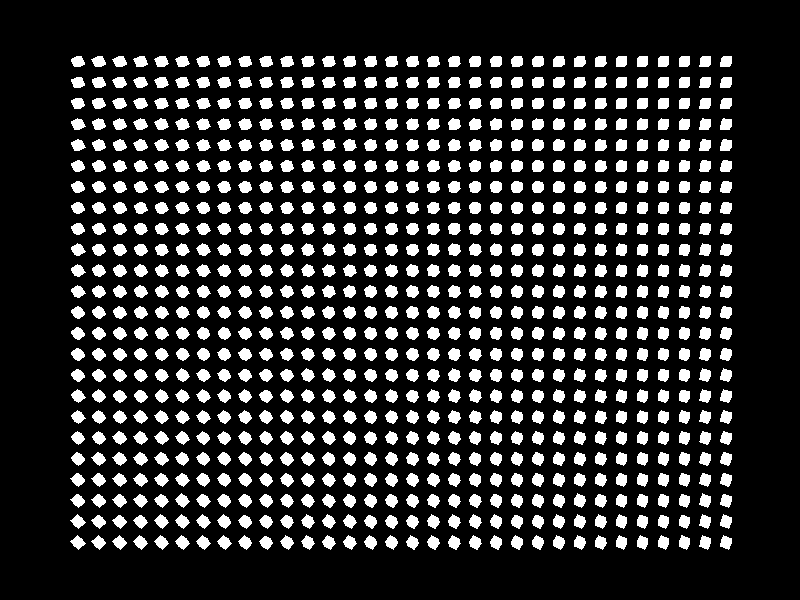
\includegraphics[width=10cm]{images/TestScene9.png}
			\caption{Output of TestScene9}
			\label{fig:TestScene9}
		\end{figure}

		We have created a ``wall'' consisting of $32 * 24 = 768$ cubes facing the camera. The frame rate is again marginally higher with the added software layer, but we couldn't find the cause for this difference in this scene. It is possible that another choice of a default value effects the performance.

		\begin{table}[htpb]
			\center
			\caption{Performance metrics for TestScene9}
			\begin{tabular}{l | l | l | l}
				& without PURGE & with PURGE & relative value\\ \hline
				Frames per second & 37.58 & 37.74 & 100.43\%\\
				Peak memory usage & 67708 & 67702 & 99.99\%\\
			\end{tabular}
			\label{tbl:Performance9}
		\end{table}

	\subsection{TestScene10: Rotating many objects}

		The same objects that were created during the previous test were rotated 360\degree around their up axis throughout the run-time. This test shows that the transmission of changes from PURGE to Ogre3d contains another big performance impact. In contrast to the previous performance deficit in TestScene8, this use case could be much more common and the solution is not as simple.
		
		\begin{table}[htpb]
			\center
			\caption{Performance metrics for TestScene10}
			\begin{tabular}{l | l | l | l}
				& without PURGE & with PURGE & relative value\\ \hline
				Frames per second & 73.96 & 30.38 & 41.08\%\\
				Peak memory usage & 79962 & 83694 & 104.67\%\\
			\end{tabular}
			\label{tbl:Performance10}
		\end{table}

		One possible optimization is sharing of attitude objects. If PURGE has the same handedness of its coordinate system as the underlying graphics engine, it would be possible to write all attitude changes into the quaternion of the underlying engine -- or binding the quaternion used by Ogre3d to the object created by PURGE. The same approach could be applied to other properties (like position and scale) as well. This solution breaks the separation of the two graphic engines in favor of a higher frame rate.

		Taking the idea of such a sacrifice of separation further, we could implement the newly created API for Ogre3d, rather than a dedicated software layer. This would eliminate the need to transmit any changes from one engine to another, leading to much higher performance.

	\subsection{TestScene11: Many objects, with a higher scene graph level}

		The layout of the test with distributed objects was repeated, this time attaching the objects in each row to a common parent node in both implementations. The consistent improvement of the frame rate now starts to indicate a positive impact of our layer on scenes consisting of multiple immobile objects, even after re-running the tests.

		\begin{table}[htpb]
			\center
			\caption{Performance metrics for TestScene11}
			\begin{tabular}{l | l | l | l}
				& without PURGE & with PURGE & relative value\\ \hline
				Frames per second & 40.22 & 40.33 & 100.28\%\\
				Peak memory usage & 67699 & 67698 & 100.00\%\\
			\end{tabular}
			\label{tbl:Performance11}
		\end{table}

		This effect proved to be the result of the model used in the tests. The results changed as we switched from dynamically created cube models to a pre-calculated cube model loaded from a file. The repeated test summarized in Table \ref{tbl:Performance11.1} has slightly lower frame rates than the previous test run, as the pre-calculated cube was larger than the dynamically created one.

		\begin{table}[htpb]
			\center
			\caption{Performance metrics for TestScene11.1}
			\begin{tabular}{l | l | l | l}
				& without PURGE & with PURGE & relative value\\ \hline
				Frames per second & 34.36 & 33.92 & 98.72\%\\
				Peak memory usage & 67700 & 67958 & 100.38\%\\
			\end{tabular}
			\label{tbl:Performance11.1}
		\end{table}

	\subsection{TestScene12: Rotating the scene nodes}

		The scene nodes containing each row are rotated around their ``up'' axis again. % The repeated communication of the state changes causes a performance loss, as in TestScene10.

		\begin{table}[htpb]
			\center
			\caption{Performance metrics for TestScene12}
			\begin{tabular}{l | l | l | l}
				& without PURGE & with PURGE & relative value\\ \hline
				Frames per second & 79.01 & 74.24 & 93.96\%\\
				Peak memory usage & 79966 & 80495 & 100.66\%\\
			\end{tabular}
			\label{tbl:Performance12}
		\end{table}

